\documentclass{standalone}
\usepackage{tikz}
\usetikzlibrary{arrows.meta, positioning, shapes}

\begin{document}
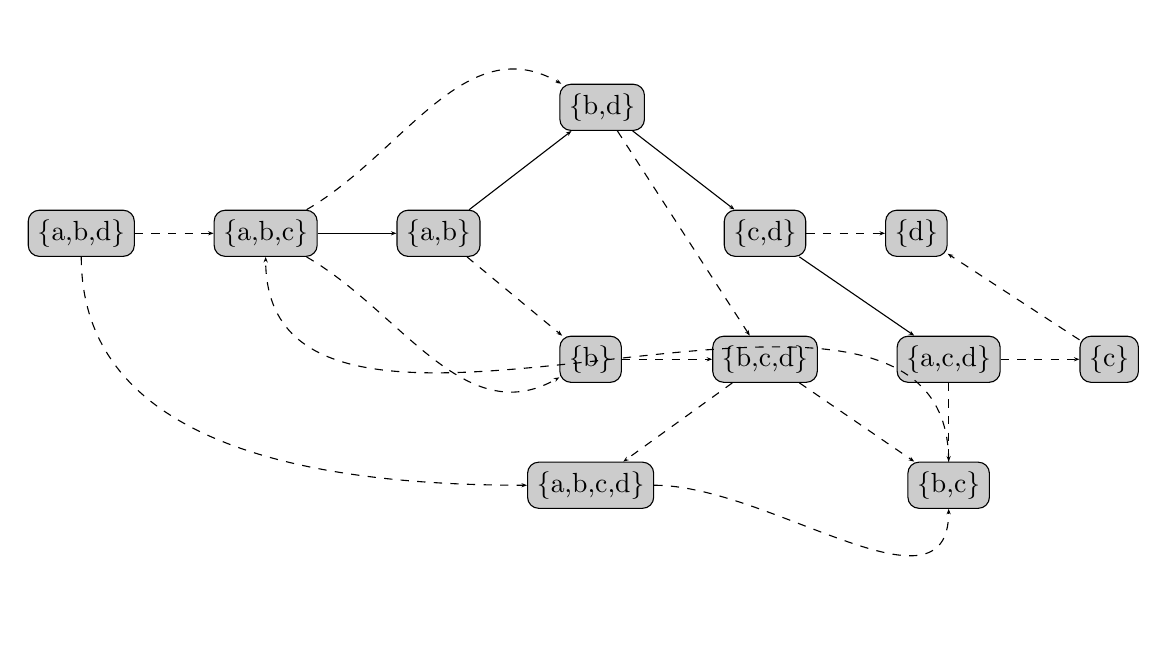
\begin{tikzpicture}[
    node/.style={draw, rounded corners, fill=gray!40, minimum size=1em},
    >={Stealth[length=2pt]},
    edge_solid/.style={->},
    edge_dashed/.style={->, dashed}
]

% Nodes
\node[node] (1) {\{a,b,d\}};
\node[node, right=of 1] (2) {\{a,b,c\}};
\node[node, right=of 2] (3) {\{a,b\}};
\node[node, above right=of 3] (4) {\{b,d\}};
\node[node, below right=of 3] (5) {\{b\}};
\node[node, below right=of 4] (6) {\{c,d\}};
\node[node, right=of 6] (7) {\{d\}};
\node[node, below=of 6] (8) {\{b,c,d\}};
\node[node, right=of 8] (9) {\{a,c,d\}};
\node[node, right=of 9] (10) {\{c\}};
\node[node, below=of 5] (11) {\{a,b,c,d\}};
\node[node, below=of 9] (12) {\{b,c\}};

% Edges
\draw[edge_dashed] (1) -- (2);
\draw[edge_solid] (2) -- (3);
\draw[edge_solid] (3) -- (4);
\draw[edge_dashed] (3) -- (5);
\draw[edge_dashed] (2) to[out=30, in=150] (4);
\draw[edge_dashed] (2) to[out=-30, in=210] (5);
\draw[edge_solid] (4) -- (6);
\draw[edge_dashed] (4) -- (8);
\draw[edge_dashed] (5) -- (8);
\draw[edge_dashed] (6) -- (7);
\draw[edge_solid] (6) -- (9);
\draw[edge_dashed] (8) -- (11);
\draw[edge_dashed] (8) -- (12);
\draw[edge_dashed] (9) -- (10);
\draw[edge_dashed] (9) -- (12);
\draw[edge_dashed] (1) to[out=-90, in=180] (11);
\draw[edge_dashed] (11) to[out=0, in=-90] (12);
\draw[edge_dashed] (12) to[out=90, in=-90] (2);
\draw[edge_dashed] (10) -- (7);

\end{tikzpicture}
\end{document}